% This file was created (at least in part) by the script ParseMdtoLatex by Louis du Plessis
% (Available from https://github.com/taming-the-beast)

\documentclass[11pt]{article}
%%%%%%%%%%%%%%%%%%%%%%%%%%%%%%%%%%%%%%%%%%%%%%%%%%%%%%%%%%%%%%%
% DO NOT EDIT THIS FILE UNLESS YOU KNOW WHAT YOU ARE DOING!!! %
%%%%%%%%%%%%%%%%%%%%%%%%%%%%%%%%%%%%%%%%%%%%%%%%%%%%%%%%%%%%%%%

\usepackage[]{authblk}
\usepackage{graphicx}
\usepackage{color}
\usepackage{longtable}
\usepackage{hanging}
\usepackage{indentfirst}
\usepackage{setspace}
\usepackage{enumitem}
\usepackage{verbatim}
\usepackage{upgreek}
\usepackage{framed}
\usepackage{textcomp}
\usepackage{url}
\usepackage{soul}
\usepackage{amsmath, amsfonts,amssymb,mathrsfs}
\usepackage{fancyhdr}
\usepackage[compact]{titlesec}
\usepackage[T1]{fontenc}
\usepackage{lmodern}

\usepackage[backend=bibtex,hyperref=true,citestyle=authoryear,bibstyle=authortitle,firstinits=true,terseinits=true,doi=false,url=false,eprint=false,maxbibnames=10,maxcitenames=2]{biblatex}
\DeclareCiteCommand{\cite}
  {\usebibmacro{prenote}}
  {\usebibmacro{citeindex}%
   \printtext[bibhyperref]{\usebibmacro{cite}}}
  {\multicitedelim}
  {\usebibmacro{postnote}}

\DeclareCiteCommand*{\cite}
  {\usebibmacro{prenote}}
  {\usebibmacro{citeindex}%
   \printtext[bibhyperref]{\usebibmacro{citeyear}}}
  {\multicitedelim}
  {\usebibmacro{postnote}}

\DeclareCiteCommand{\parencite}[\mkbibparens]
  {\usebibmacro{prenote}}
  {\usebibmacro{citeindex}%
    \printtext[bibhyperref]{\usebibmacro{cite}}}
  {\multicitedelim}
  {\usebibmacro{postnote}}

\DeclareCiteCommand*{\parencite}[\mkbibparens]
  {\usebibmacro{prenote}}
  {\usebibmacro{citeindex}%
    \printtext[bibhyperref]{\usebibmacro{citeyear}}}
  {\multicitedelim}
  {\usebibmacro{postnote}}

\DeclareCiteCommand{\footcite}[\mkbibfootnote]
  {\usebibmacro{prenote}}
  {\usebibmacro{citeindex}%
  \printtext[bibhyperref]{ \usebibmacro{cite}}}
  {\multicitedelim}
  {\usebibmacro{postnote}}

\DeclareCiteCommand{\footcitetext}[\mkbibfootnotetext]
  {\usebibmacro{prenote}}
  {\usebibmacro{citeindex}%
   \printtext[bibhyperref]{\usebibmacro{cite}}}
  {\multicitedelim}
  {\usebibmacro{postnote}}

\DeclareCiteCommand{\textcite}
  {\boolfalse{cbx:parens}}
  {\usebibmacro{citeindex}%
   \printtext[bibhyperref]{\usebibmacro{textcite}}}
  {\ifbool{cbx:parens}
     {\bibcloseparen\global\boolfalse{cbx:parens}}
     {}%
   \multicitedelim}
  {\usebibmacro{textcite:postnote}}

\newcommand{\citep}{\parencite}
\newcommand{\citet}{\textcite}
\defbibheading{relevref}[\refname]{\section*{Relevant References}}

\renewcommand{\postnotedelim}{\iffieldpages{postnote}{\addcolon}{\addcomma\space}} 
\DeclareFieldFormat{postnote}{#1} 

\DeclareFieldFormat[article, inbook, incollection, inproceedings, patent, thesis, unpublished]{title}{#1}
\DeclareFieldFormat[article, inbook, incollection, inproceedings, patent, thesis, unpublished]{journaltitle}{\mkbibemph{#1}\nopunct}
\DeclareFieldFormat[article, inbook, incollection, inproceedings, patent, thesis, unpublished]{volume}{{#1}\addcolon} %puts volume number in parens
%\DeclareFieldFormat[article, inbook, incollection, inproceedings, patent, thesis, unpublished]{year}{\mkbibparens{#1}\nopunct} %puts year in parens

\DeclareFieldFormat[article, incollection, patent, thesis, unpublished]{pages}{{\nopp#1}}

\DeclareFieldFormat{sentencecase}{\MakeSentenceCase{#1}}

\renewbibmacro*{title}{%
  \ifthenelse{\iffieldundef{title}\AND\iffieldundef{subtitle}}
    {}
    {\ifthenelse{\ifentrytype{article}\OR\ifentrytype{inbook}%
      \OR\ifentrytype{incollection}\OR\ifentrytype{inproceedings}%
      \OR\ifentrytype{inreference}}
      {\printtext[title]{%
        \printfield[sentencecase]{title}%
        \setunit{\subtitlepunct}%
        \printfield[sentencecase]{subtitle}}}%
      {\printtext[title]{%
        \printfield[titlecase]{title}%
        \setunit{\subtitlepunct}%
        \printfield[titlecase]{subtitle}}}%
     \newunit}%
  \printfield{titleaddon}}

\DefineBibliographyStrings{english}{% various adjustments to common bib entry strings
urlseen = {Accessed:},% What goes in front of the date a URL was accessed/retrieved etc.
editor = {(Ed)},%Ed – no dot, in brackets
editors = {(Eds)},% Eds – no dot, in brackets
byeditor = {(Ed.)}}% ‘Edited by’ for edited works

\DeclareNameAlias{default}{last-first}

\renewbibmacro{in:}{}

\renewbibmacro{publisher+location+date}{
  \iflistundef{publisher}
    {}
    {\printlist{publisher}%
       {\addcomma\space}%
      \iflistundef{location}
        {}
        {\printlist{location}}%
    }
}

\DeclareBibliographyDriver{article}{%
\usebibmacro{bibindex}%
\usebibmacro{begentry}%
\usebibmacro{author/translator+others}%
\newunit\newblock
\printfield{year}%
\setunit{\labelnamepunct}\newblock
\usebibmacro{title}%
\newunit
\printlist{language}%
\newunit\newblock
\usebibmacro{byauthor}%
\newunit\newblock
\usebibmacro{bytranslator+others}%
\newunit\newblock
\printfield{version}%
\newunit\newblock
%\usebibmacro{in:}% %mit in:
\usebibmacro{journal}%
\newunit\newblock
\printfield{volume}%
\newunit\newblock
\usebibmacro{byeditor+others}%
\newunit\newblock
\usebibmacro{note+pages}%
\newunit\newblock
\iftoggle{bbx:isbn}
{}%
\newunit\newblock
\usebibmacro{doi+eprint+url}%
\newunit\newblock
\usebibmacro{addendum+pubstate}%
\newunit\newblock
\usebibmacro{pageref}%
\usebibmacro{finentry}}

\DeclareBibliographyDriver{inproceedings}{%
\usebibmacro{bibindex}%
\usebibmacro{begentry}%
\usebibmacro{author/translator+others}%
\newunit\newblock
\printfield{year}%
\setunit{\labelnamepunct}\newblock
\usebibmacro{title}%
\newunit
\printlist{language}%
\newunit\newblock
\usebibmacro{byauthor}%
\newunit\newblock
\usebibmacro{bytranslator+others}%
\newunit\newblock
\printfield{version}%
\newunit\newblock
%\usebibmacro{in:}% %mit in:
\usebibmacro{booktitle}%
\newunit\newblock
\printfield{volume}%
\newunit\newblock
\usebibmacro{byeditor+others}%
\newunit\newblock
\usebibmacro{publisher+location+date}%
\newunit\newblock
\usebibmacro{note+pages}%
\newunit\newblock
\usebibmacro{pageref}%
\usebibmacro{finentry}}

\DeclareBibliographyDriver{book}{%
\usebibmacro{bibindex}%
\usebibmacro{begentry}%
\usebibmacro{author/translator+others}%
\newunit\newblock
\printfield{year}%
\setunit{\labelnamepunct}\newblock
\usebibmacro{title}%
\newunit
\printlist{language}%
\newunit\newblock
\usebibmacro{byauthor}%
\newunit\newblock
\usebibmacro{bytranslator+others}%
\newunit\newblock
%\usebibmacro{in:}% %mit in:
\usebibmacro{booktitle}%
\newunit\newblock
\printfield{volume}%
\newunit\newblock
\usebibmacro{publisher+location+date}%
\newunit\newblock
\usebibmacro{note+pages}%
\newunit\newblock
\usebibmacro{pageref}%
\usebibmacro{finentry}}




\setlist{nolistsep}

\setlength{\evensidemargin}{0in}
\setlength{\headheight}{0in}
\setlength{\headsep}{0in}
\setlength{\oddsidemargin}{-0.25in}
\setlength{\paperheight}{11in}
\setlength{\paperwidth}{8.5in}
\setlength{\tabcolsep}{0in}
\setlength{\textheight}{9in}
\setlength{\textwidth}{7in}
\setlength{\topmargin}{0in}
\setlength{\topskip}{0in}
\setlength{\voffset}{0in}
\parskip = 0.15in
\pagestyle{plain}
\setlength{\parindent}{0cm}

\definecolor{citescol}{RGB}{194,101,1}
\definecolor{urlscol}{RGB}{0,150,206}
\definecolor{linkscol}{RGB}{149,0,207}
\definecolor{mycol}{RGB}{25,23,191}
\definecolor{outputcol}{RGB}{34,139,34}
\definecolor{tcol}{RGB}{165,0,14}


\DeclareMathAlphabet{\msfsl}{T1}{cmr}{m}{it}
\DeclareMathAlphabet{\msyf}{OMX}{pcr}{m}{it}
\newcommand{\alf}{\upalpha}
\newcommand{\hilight}[1]{\colorbox{yellow}{#1}}

\newcommand{\levelone}[1]{
\bigskip
\noindent{\LARGE{\textsc{#1}}}
\vspace {0.05in}
}

\newcommand{\leveltwo}[1]{
\bigskip
\noindent{\Large{\textit{#1}}}
\vspace {-1mm}
}

\newcommand{\descriptionhead}[1]{
\noindent{\textcolor{mycol}{\textbf{\textit{#1}}}}\\ \vspace{-7mm}
}

\newcommand{\dhead}[1]{
\noindent{\textbf{\textit{#1 --}}}
}



\newcommand{\exs}[1]{
\vspace{-4mm}
\begin{itemize}
\item #1 \\ \vspace{-8mm}
\end{itemize}
}

\newcommand{\nbo}[1]{{\color{red}{#1}}}


\newcommand{\stepbullet}{\noindent \textbullet \ }
\newcommand{\mi}[1]{\textbf{\textit{#1}}}


\newcommand{\levelthree}[1]{\textit{#1 --}}


%\bibliographystyle{apalike}
%\bibpunct[; ]{(}{)}{;}{a}{,}{;}


\usepackage[breaklinks]{hyperref}
\usepackage[all]{hypcap}
\hypersetup{colorlinks=true,linkcolor=linkscol,citecolor=citescol,urlcolor=urlscol}


\newcommand{\R}{\texttt{R} }
\newcommand{\TESS}{\texttt{TESS}}
\newcommand{\PBD}{\texttt{PBD}}
\newcommand{\DDD}{\texttt{DDD}}
\newcommand{\Laser}{\texttt{laser}}
\newcommand{\TreePar}{\texttt{TreePar}}
\newcommand{\diversitree}{\texttt{diversitree}}
\newcommand{\RevBayes}{\texttt{RevBayes}}
\newcommand{\Rev}{\texttt{Rev}}
\newcommand{\MrBayes}{\texttt{MrBayes}}
\newcommand{\BEAST}{\texttt{BEAST}}
\newcommand{\PhyloBayes}{\texttt{PhyloBayes}}
\newcommand{\PAML}{\texttt{PAML}}

\let\otheriint\iint
\let\iint\relax
\usepackage{ wasysym }

\usepackage{framed}
\usepackage[]{listings}
%\usepackage{fontspec}
\usepackage{placeins}
\usepackage{epstopdf}



\lstset{backgroundcolor=\color[rgb]{0.972,0.972,0.972},
		tabsize=4,
		rulecolor=,
        basicstyle=\scriptsize,
        upquote=true,
        aboveskip={1.5\baselineskip},
        columns=fixed,
        showstringspaces=false,
        extendedchars=true,
        breaklines=true,
        prebreak = \raisebox{0ex}[0ex][0ex]{\ensuremath{\hookleftarrow}},
        frame=single,
        showtabs=false,
        showspaces=false,
        showstringspaces=false,
        identifierstyle=\ttfamily,
        keywordstyle=\color[rgb]{0,0,1},
        commentstyle=\color[rgb]{0.133,0.545,0.133},
        stringstyle=\color[rgb]{0.627,0.126,0.941}
}

\definecolor{shadecolor}{RGB}{194,225,255}

\setlength{\tabcolsep}{5pt}
\setlength{\topmargin}{-0.4in}
\setlength{\headheight}{14.5pt}
\pagestyle{fancy}

\newcommand{\taha}[1]{{\textcolor{red}{[TAH comment: #1]}}} % TAH comment

\titlespacing{\section}{0pt}{*0}{*0}
\titlespacing{\subsection}{0pt}{*0}{*0}
\titlespacing{\subsubsection}{0pt}{*0}{*0}

\titleformat{\section}
  {\normalfont\Large\bfseries\color{mycol}}
  {\thesection}{1em}{}

\titleformat{\subsection}
  {\normalfont\large\bfseries\color{mycol}}
  {\thesubsection}{1em}{}

\titleformat{\subsubsection}
  {\normalfont\bfseries\color{mycol}}
  {\thesubsubsection}{1em}{}

% command for MrBayes command-line step
\newcommand{\cl}[1]{{\texttt{\textbf{#1}}}}

\newcommand{\colx}[1]{{\textcolor{tcol}{#1}}}

\newcommand{\mbcl}[1]{\exs{\cl{MrBayes > {#1}}}}

\newcommand{\rbprmt}{RevBayes > } 
\newcommand{\rbcl}[1]{\exs{\cl{\rbprmt{#1}}}}
\newcommand{\rbout}[1]{\exs{\cl{\textcolor{outputcol}{#1}}}}
\newcommand{\rbdn}{{\Large \symbol{126}}} % This makes a copy/pasteable tilde
\newcommand{\rbclml}[1]{\exs{\cl{\ \ \ \ \ \ \ \ \ \ \ {#1}}}}

% text box settings
% requires compiling w/ XeLaTeX
%\newfontfamily\listingsfont[Scale=1.0]{Courier New}
%\lstset{basicstyle=\listingsfont, columns=texcl}
%\defaultfontfeatures{Mapping=tex-text}


\makeatletter
\lst@CCPutMacro\lst@ProcessOther {"2D}{\lst@ttfamily{-{}}{-{}}}
\@empty\z@\@empty
\makeatother


\usepackage{tikz}

\setlength{\topmargin}{-0.4in}
\setlength{\headheight}{14.5pt}
\pagestyle{fancy}

\usepackage[breaklinks]{hyperref}
\usepackage[all]{hypcap}
\hypersetup{colorlinks=true,linkcolor=linkscol,citecolor=citescol,urlcolor=urlscol}

\definecolor{lg}{gray}{0.75}
\def\gcirc{{%
    \setbox0\hbox{$\fullmoon$}%
    \rlap{\hbox to \wd0{\hss{$\textcolor{lg}{\newmoon}$}\hss}}\box0
}}



% Add your bibtex library here
\addbibresource{master-refs.bib}


%%%%%%%%%%%%%%%%%%%%
% Do NOT edit this %
%%%%%%%%%%%%%%%%%%%%
\begin{document}
\renewcommand{\headrulewidth}{0.5pt}
\headsep = 20pt
\lhead{ }
\rhead{\textsc {BEAST v2 Tutorial}}
\thispagestyle{plain}


%%%%%%%%%%%%%%%%%%
% Tutorial title %
%%%%%%%%%%%%%%%%%%
\begin{center}

	% Enter the name of your tutorial here
	\textbf{\LARGE Tutorial using BEAST v2.7.x}\\\vspace{2mm}

	% Enter a short description of your tutorial here
	\textbf{\textcolor{mycol}{\Large The ClaDS package}}\\

	\vspace{4mm}

	% Enter the names of all the authors here
	{\Large {\em Joëlle Barido-Sottani}}
\end{center}

Inferring progressive changes in birth and death rates

%%%%%%%%%%%%%%%%%
% Tutorial body %
%%%%%%%%%%%%%%%%%

\hypertarget{background}{%
\section{Background}\label{background}}

This tutorial will show how to configure and run a model with
progressive changes in birth and death rates, using the ClaDS tree prior
implemented in the BEAST2 package ClaDS.

The Cladogenetic Diversification rate Shift (ClaDS) model is a
birth-death process which is designed to represent gradual, progressive
changes in rates throughout a phylogeny. It is similar in principle to
an autocorrelated clock model, as new birth and death rates are drawn
for each edge from a distribution which depends on the ancestral rates.

As an example, we consider a lineage \passthrough{$ N $},
with its associated birth rate \passthrough{$ \lambda_N $}
and death rate \passthrough{$ \mu_N $}. At the next birth
event, the lineage \passthrough{$ N $} splits into lineages
\passthrough{$ N^\prime $} and
\passthrough{$ N^{\prime\prime} $}. The new birth rates
\passthrough{$ \lambda_N^\prime $} and
\passthrough{$ \lambda_N^{\prime\prime} $} are drawn
from a lognormal distribution with mean
\passthrough{$ M = \log(\alpha \times \lambda_N ) $}
and standard deviation \passthrough{$ S = \sigma $}. The
model parameters \passthrough{$ \alpha $},
\passthrough{$ \sigma $}, and the birth rate at the root,
\passthrough{$ \lambda_0 $}, can be estimated by the
inference.

The package includes two separate options for sampling the death rate:
1. New death rates are not sampled separately, but controlled by the
turnover parameter \passthrough{$ \epsilon $}, which is the
same throughout the phylogeny and can be estimated by the inference.
Thus for each lineage \passthrough{$ N $}, we have
\passthrough{$ \mu_N = \epsilon \times \lambda_N $}.
This is the parametrization by default. 2. New death rates are sampled
from the ancestral rates, following a similar lognormal distribution to
the birth rates. Thus, for lineage \passthrough{$ N $} with
descendants \passthrough{$ N^\prime $} and
\passthrough{$ N^{\prime\prime} $}, we draw the new
death rates \passthrough{$ \mu_N^\prime $} and
\passthrough{$ \mu_N^{\prime\prime} $} from a
lognormal distribution with mean
\passthrough{$ M = \log(\alpha_M \times \mu_N ) $} and
standard deviation \passthrough{$ S = \sigma_M $}. In this
case and similar to the birth rate,
\passthrough{$ \alpha_M $},
\passthrough{$ \sigma_M $}, and the death rate at the
root, \passthrough{$ \mu_0 $}, are parameters of the model
and can be estimated by the inference. The choice of death rate
parametrization is left to the user, and will depend on the dataset and
on which characteristics are thought to drive the variations in rate.
The first parametrization is appropriate when the variations of both
rates are tied to the same factor and thus strongly correlated, whereas
the second parametrization is more appropriate when the variations in
birth rates and death rates are uncorrelated. The first parametrization
is also more simple and contains less parameters, and thus may be easier
to use when the available data is limited.

Finally, it is also possible to set either the birth rate or the death
rate to be constant throughout the phylogeny, by setting the
corresponding trend parameter \passthrough{$ \alpha $} or
\passthrough{$ \alpha_M $} to 1 and the corresponding
standard deviation parameter \passthrough{$ \sigma $} or
\passthrough{$ \sigma_M $} to 0. This will lead to
\passthrough{$ \lambda_N = \lambda_0 $} or
\passthrough{$ \mu_N = \mu_0 $} for all lineages.

More details on the model and an evaluation of its performance in
various conditions can be found in the original publication
\citep{Maliet2019}. The specific implementation of ClaDS as a BEAST2
package is presented in a separate article \citep{ClaDS2022}. \clearpage

\hypertarget{programs-used-in-this-exercise}{%
\section{Programs used in this
Exercise}\label{programs-used-in-this-exercise}}

\hypertarget{beast2---bayesian-evolutionary-analysis-sampling-trees-2}{%
\subsubsection{BEAST2 - Bayesian Evolutionary Analysis Sampling Trees
2}\label{beast2---bayesian-evolutionary-analysis-sampling-trees-2}}

BEAST2 is a free software package for Bayesian evolutionary analysis of
molecular sequences using MCMC and strictly oriented toward inference
using rooted, time-measured phylogenetic trees \citep{Bouckaert2019}.
This tutorial uses BEAST2 version 2.6, however the ClaDS package is also
available for BEAST2 version 2.7 and works the same way.

\hypertarget{beauti-bayesian-evolutionary-analysis-utility}{%
\subsubsection{BEAUti -- Bayesian Evolutionary Analysis
Utility}\label{beauti-bayesian-evolutionary-analysis-utility}}

BEAUti is a utility program with a graphical user interface for creating
BEAST2 input files, which are written in XML. The eXtensible Markup
Language (XML) is a general-purpose markup language, which allows for
the combination of text and additional information. The use of the XML
makes analysis specification very flexible and readable by both the
program and people. The XML file specifies all the components of the
analysis, including sequences, node calibrations, models, priors, output
file names.

\hypertarget{treeannotator}{%
\subsubsection{TreeAnnotator}\label{treeannotator}}

TreeAnnotator is used to summarize the posterior sample of trees to
produce a maximum clade credibility tree and summarize the posterior
estimates of other parameters that can be easily visualized on the tree
(e.g.~node height). This program is also useful for comparing a specific
tree topology and branching times to the set of trees sampled in the
MCMC analysis.

\hypertarget{tracer}{%
\subsubsection{Tracer}\label{tracer}}

Tracer is used for assessing and summarizing the posterior estimates of
the various parameters sampled by the Markov Chain. This program can be
used for visual inspection and assessment of convergence and it also
calculates 95\% credible intervals (which approximate the 95\% highest
posterior density intervals) and effective sample sizes (ESS) of
parameters. Contrary to the other software in this section, Tracer is
not distributed with BEAST2 and needs to be downloaded separately
\href{http://beast.community/tracer}{here}. \clearpage

\hypertarget{practical-lineage-specific-birth-and-death-rate-inference-under-the-clads-model}{%
\section{Practical: Lineage-specific Birth and Death Rate Inference
Under the ClaDS
Model}\label{practical-lineage-specific-birth-and-death-rate-inference-under-the-clads-model}}

\hypertarget{dataset}{%
\subsection{Dataset}\label{dataset}}

The dataset used in this tutorial is an alignment of sequences sampled
from twelve primate species, also used in the Introduction tutorial.

\hypertarget{setting-up-the-xml-file}{%
\subsection{Setting up the XML file}\label{setting-up-the-xml-file}}

This section will demonstrate how to create an XML configuration file
using BEAUti, which will then be used to run the analysis in BEAST2.

\hypertarget{package-installation}{%
\subsubsection{Package installation}\label{package-installation}}

The first step is to install the ClaDS package, which will allow us to
set up and run an analysis with lineage-specific birth and death rates.

\begin{framed}
Launch \textbf{BEAUti}, then open the \textbf{BEAST2 Package Manager} by
navigating to \textbf{File \textgreater{} Manage Packages}. (Figure
\ref{packageManage1})
\end{framed}

\begin{figure}
    \centering
    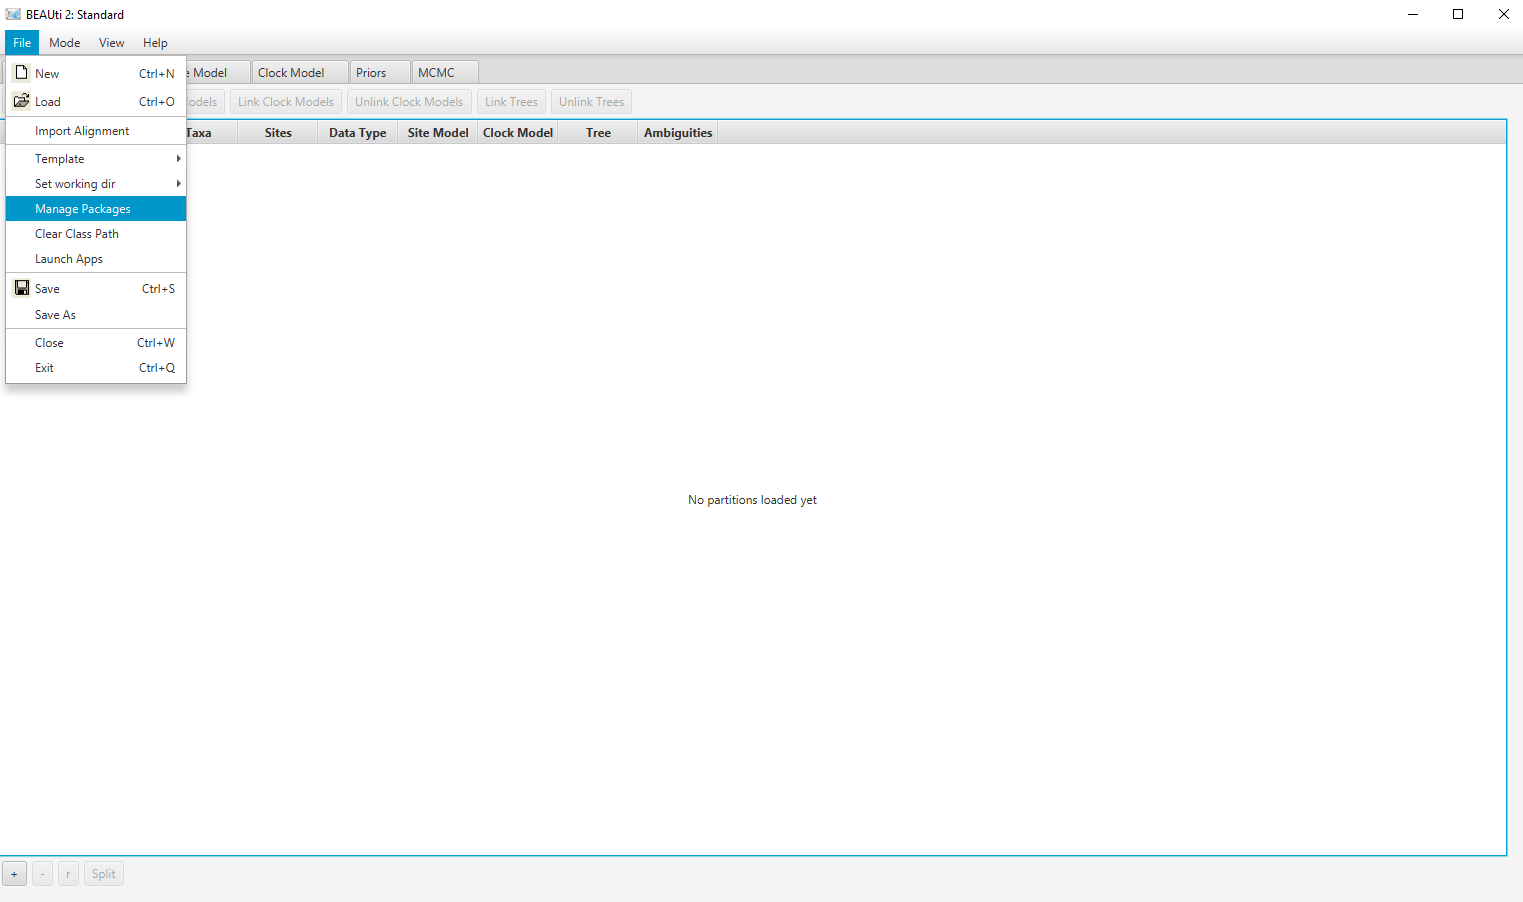
\includegraphics[width=0.800000\textwidth]{figures/package_manager.png}
    \caption{Finding the BEAST2 Package Manager.}
    \label{packageManage1}
\end{figure}

\begin{framed}
Install the \textbf{ClaDS} package by selecting it and clicking the
\textbf{Install/Upgrade} button. (Figure \ref{packageManage2})
\end{framed}

\begin{figure}
    \centering
    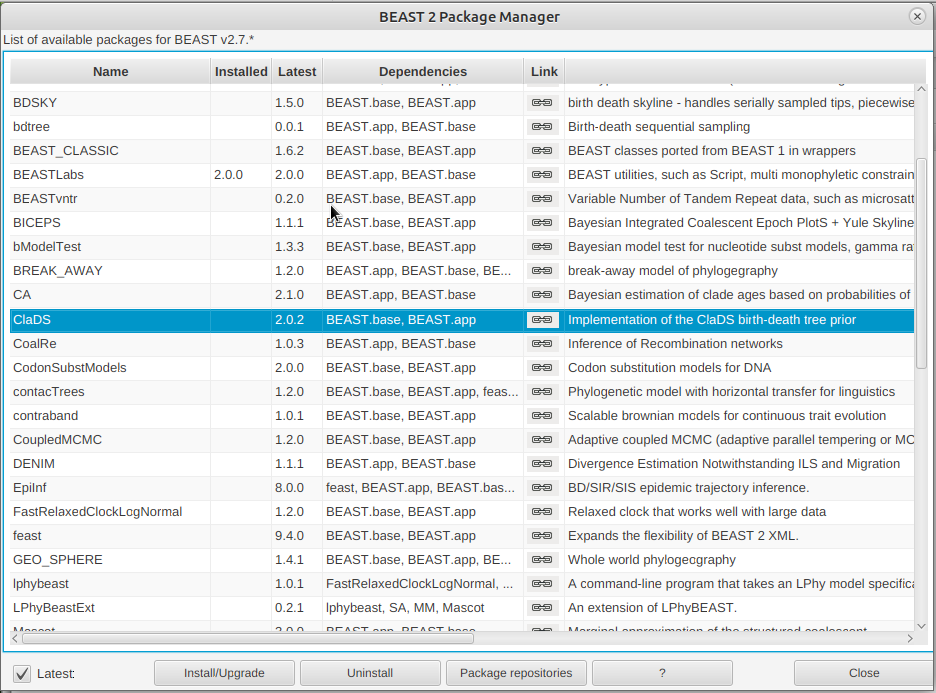
\includegraphics[width=0.700000\textwidth]{figures/packageClaDS.png}
    \caption{The BEAST2 Package Manager.}
    \label{packageManage2}
\end{figure}

BEAUti needs to be restarted for the newly installed package to be
loaded properly.

\begin{framed}
Close the \textbf{BEAST2 Package Manager} and \textbf{\emph{restart}}
BEAUti to fully load the \textbf{ClaDS} package.
\end{framed}

\hypertarget{setting-the-templates}{%
\subsubsection{Setting the templates}\label{setting-the-templates}}

BEAUti uses templates to define specific model configurations. The ClaDS
template needs to be selected to set up an analysis using the ClaDS
model.

\begin{framed}
Select the \textbf{ClaDS template} by navigating to \textbf{File
\textgreater{} Template}. (Figure \ref{template})
\end{framed}

\begin{figure}
    \centering
    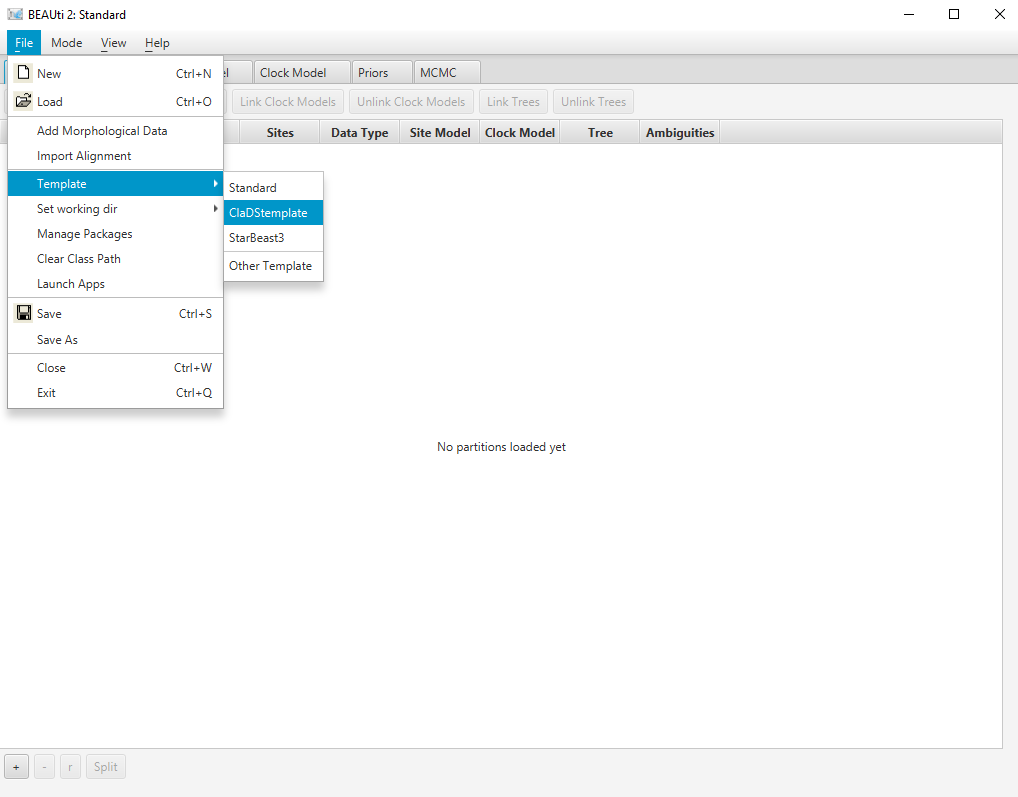
\includegraphics[width=0.800000\textwidth]{figures/template.png}
    \caption{Selecting the ClaDS template.}
    \label{template}
\end{figure}

\hypertarget{importing-the-alignment}{%
\subsubsection{Importing the alignment}\label{importing-the-alignment}}

The first step of the setup is to import the alignment that we will be
using in this analysis.

\begin{framed}
Open \textbf{BEAUti}. Navigate to \textbf{File \textgreater{} Import
Alignment} (Figure \ref{importAlignment}) and select the file
\passthrough{\lstinline!primate-mtDNA.nex!} in the data directory or
simply drag and drop the file in the \textbf{Partitions} window.
\end{framed}

\begin{figure}
    \centering
    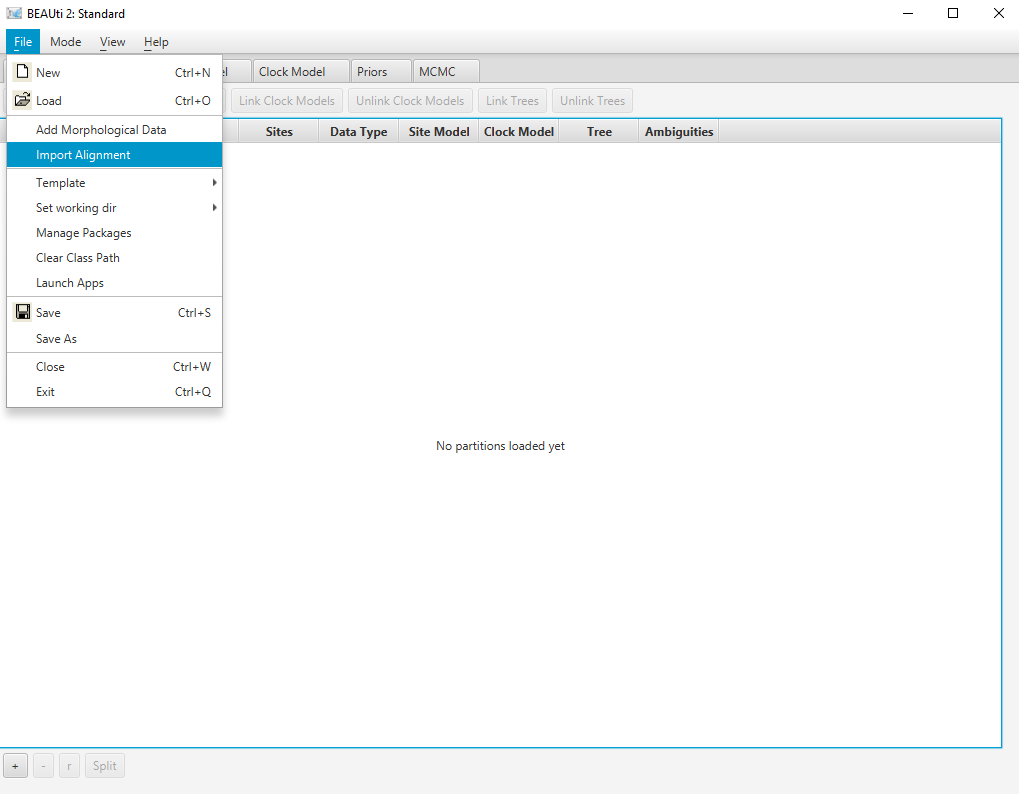
\includegraphics[width=0.800000\textwidth]{figures/alignment.png}
    \caption{Importing the alignment into BEAUti.}
    \label{importAlignment}
\end{figure}

\hypertarget{linking-the-tree-and-clock-model}{%
\subsubsection{Linking the tree and clock
model}\label{linking-the-tree-and-clock-model}}

Since we have imported an alignment containing different partitions,
BEAUti has automatically created separate substitution models, clock
models and trees for each of the partitions. We will keep the separate
substitution models, however we would like to estimate only one clock
model and one phylogeny. Thus we need to link the clock models and trees
for all partitions.

\begin{framed}
In the \textbf{Partitions} panel, select all partitions. Click on the
\textbf{Link Clock Models} button. You should see that the \textbf{Clock
Model} column now contains the same value for all partitions. Click on
the \textbf{Link trees} button. You should see that the \textbf{Tree}
column now contains the same value for all partitions. Optionally,
rename the tree and clock model to \textbf{primates} by clicking on the
name field, typing the new name then pressing \textbf{Enter}.
\end{framed}

The final alignment configuration is shown in Figure \ref{linkedModels}.

\begin{figure}
    \centering
    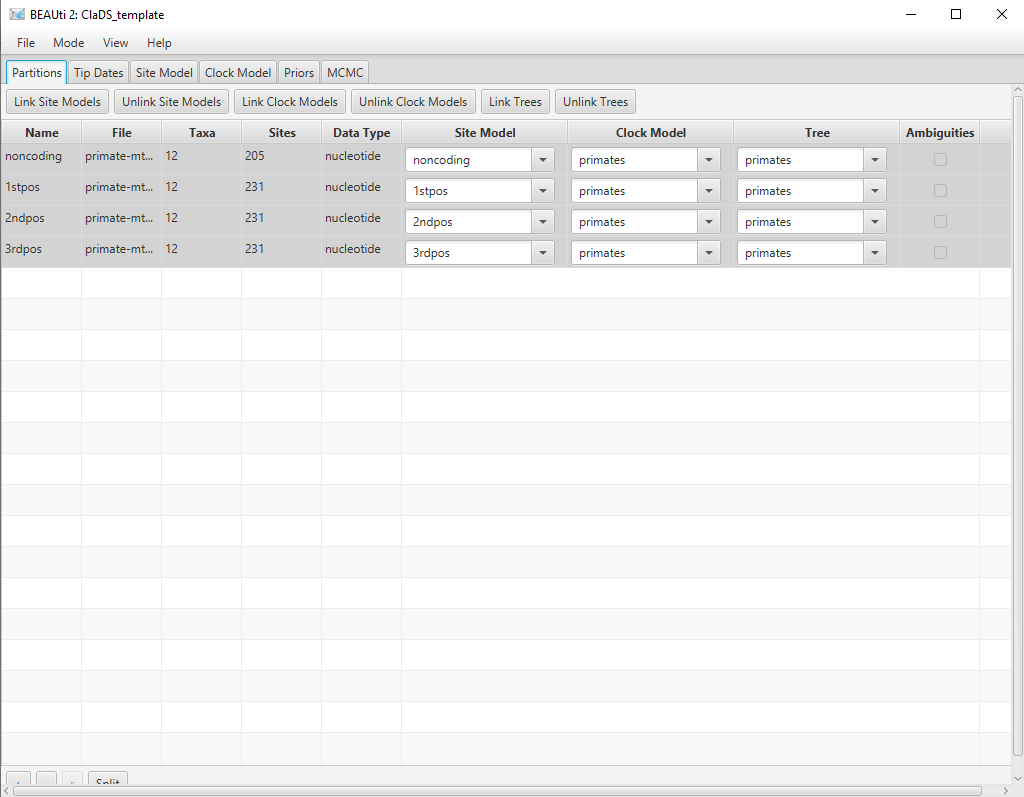
\includegraphics[width=0.800000\textwidth]{figures/linked_models.png}
    \caption{Partition panel with linked tree and clock model.}
    \label{linkedModels}
\end{figure}

\hypertarget{setting-up-the-substitution-models}{%
\subsubsection{Setting up the substitution
models}\label{setting-up-the-substitution-models}}

The next set is to set up the substitution models for each alignments,
found in the \textbf{Site Model} panel. We will set up HKY + G models
for both alignments, with the number of rate categories set to 4.

\begin{framed}
In the \textbf{Site Model} panel, set the \textbf{Gamma Category Count}
to \textbf{4}. Click on the arrow next to \textbf{JC69}, and select the
\textbf{HKY} model. Select the remaining three partitions (use
\textbf{shift+click}). Select \passthrough{\lstinline!noncoding!} and
click \textbf{OK} to to clone the site model for the other three
partitions from \passthrough{\lstinline!noncoding!}.
\end{framed}

The final substitution model configuration is shown in Figure
\ref{subst}.

\begin{figure}
    \centering
    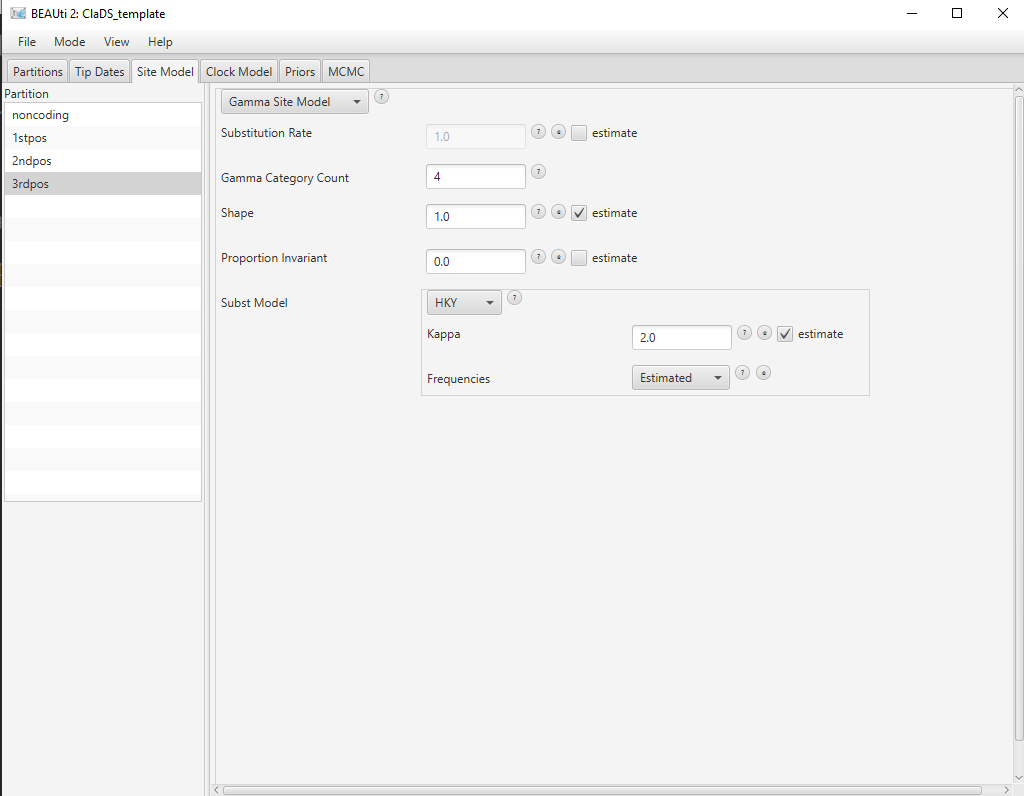
\includegraphics[width=0.800000\textwidth]{figures/subst.png}
    \caption{Site model panel with HKY+G model.}
    \label{subst}
\end{figure}

\hypertarget{setting-priors}{%
\subsubsection{Setting priors}\label{setting-priors}}

\hypertarget{adding-calibration-times}{%
\paragraph{Adding calibration times}\label{adding-calibration-times}}

The next step is to look at the different priors, in the \textbf{Priors}
panel. The default priors for most parameters are reasonable for this
dataset so we will not change them. However, we need to add calibration
times to our analysis in order to estimate the clock rate and node ages.
We will accomplish this by setting an MRCA prior, which adds a prior on
the age of the most recent common ancestor of selected tips. These
priors can also constrain certain subclades of the tree to be
monophyletic.

\begin{framed}
In the \textbf{Priors} panel, click on the \textbf{+ Add Prior} button
at the bottom of the list and select the \textbf{MRCA Prior}. This opens
the \textbf{Taxon Set Editor}. Select the taxa \textbf{Homo\_Sapiens}
and \textbf{Pan} and click on the \textbf{\textgreater\textgreater{}}
button to add them to the set. Write the name of the taxon set
\textbf{human-chimp} in the box \textbf{Taxon set label} (Figure
\ref{taxonSet}) and click \textbf{OK} to confirm.
\end{framed}

\begin{figure}
    \centering
    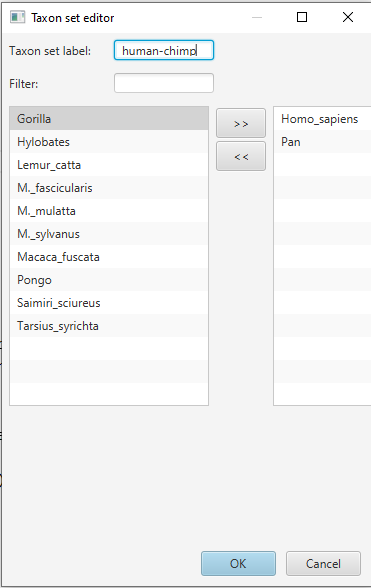
\includegraphics[width=0.400000\textwidth]{figures/taxonSet.png}
    \caption{Taxon set editor.}
    \label{taxonSet}
\end{figure}

The new prior now appears at the bottom of the list of priors, but it is
not completely configured yet. We still need to set this subclade to be
monophyletic, and select a distribution for the age of its most recent
common ancestor.

\begin{framed}
Click on the arrow on the right to \textbf{{[}none{]}} and select a
\textbf{Normal} distribution for the age of the clade. Click on the
arrow on the left of \textbf{human-chimp.prior} to open the detailed
view of the distribution. Set the \textbf{Mean} parameter of the
distribution to \textbf{6} and the \textbf{Sigma} parameter of the
distribution to \textbf{0.5} (Figure \ref{MRCApriorDet}). Click on the
arrow again to close the detailed view. Check the \textbf{monophyletic}
checkbox next to the \textbf{human-chimp.prior}.
\end{framed}

\begin{figure}
    \centering
    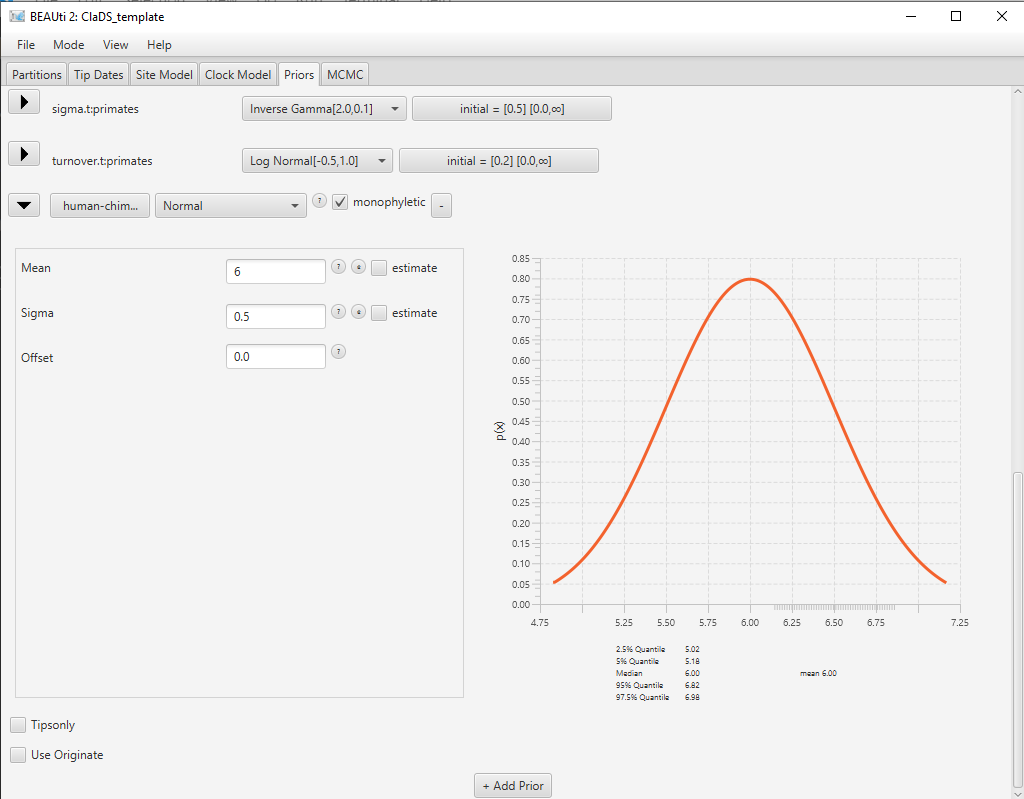
\includegraphics[width=0.800000\textwidth]{figures/MRCAprior_det.png}
    \caption{MRCA prior with age distribution.}
    \label{MRCApriorDet}
\end{figure}

You will notice that a new parameter (and prior) has been added to the
list, the mean clock rate \textbf{clockRate.c:primates}. By adding a
prior on the age of one of the nodes in the tree, we have calibrated our
time tree and BEAUti has automatically adjusted the analysis as a
result.

\hypertarget{the-tree-prior}{%
\subsubsection{The tree prior}\label{the-tree-prior}}

Next, we will take a look the tree prior, i.e.~the ClaDS model. By
default most of the parameters of the model are estimated, so it is
usually not necessary to change their starting values. However, the
extant sampling proportion (\passthrough{$ \rho $}) is
fixed, and so needs to be correct. Our dataset contains 12 taxa compared
to an estimated 414 extant species for the clade of primates, so the
correct extant sampling probability would be
\passthrough{$ \rho = 0.03 $}. But the ClaDS package
performs badly for low sampling probabilities, so for the purpose of
this exercise we will assume an extant sampling probability of
\passthrough{$ \rho = 0.3 $}.

\begin{framed}
Click on the arrow next to \textbf{Tree} to open the \textbf{ClaDS}
options. Change the value for \textbf{rho} (extant sampling proportion)
of the ClaDS model to \textbf{0.3} (Figure \ref{treePrior}).
\end{framed}

\begin{figure}
    \centering
    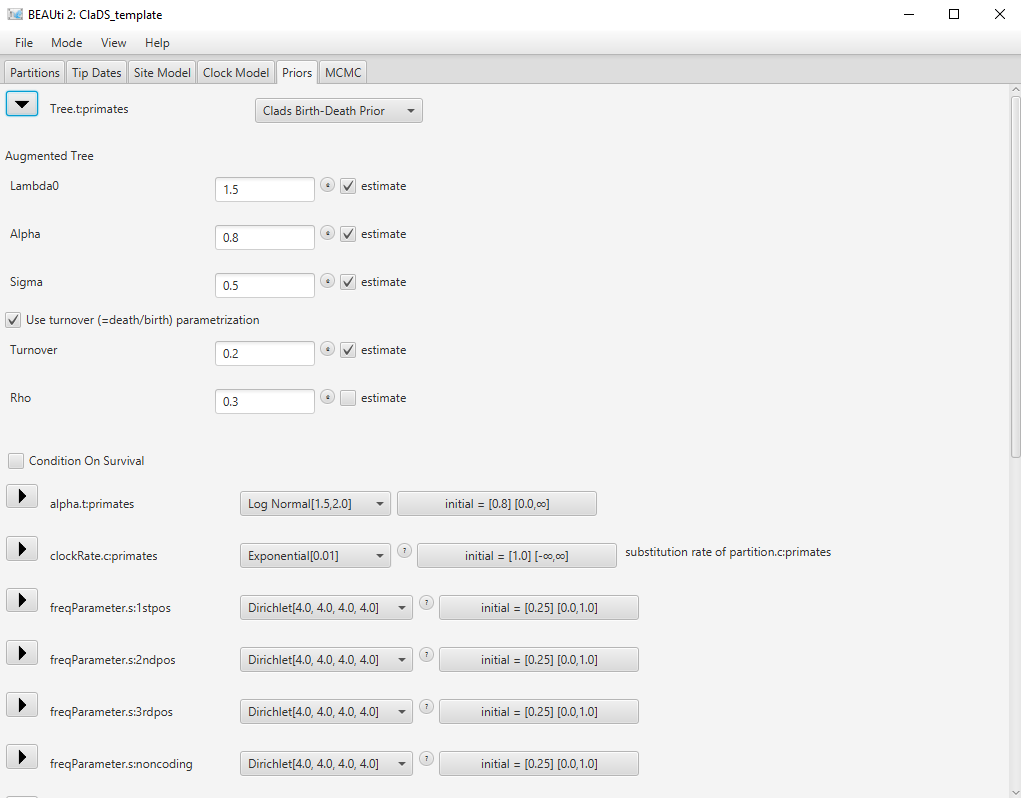
\includegraphics[width=0.800000\textwidth]{figures/treeprior.png}
    \caption{The ClaDS tree prior.}
    \label{treePrior}
\end{figure}

Note that many other options are available in this section, such as
fixing the value of some parameters (\textbf{estimate} checkboxes), or
changing the parametrization of the death rate (\textbf{Use fixed
turnover} checkbox). Our current dataset only contains extant species,
so it unlikely that we will be able to estimate the death rate
precisely. In consequence, we will set the death rate by using the
simpler constant turnover model, which is the default.

\hypertarget{the-parameter-priors}{%
\subsubsection{The parameter priors}\label{the-parameter-priors}}

Most of the default parameter priors are reasonable, so we will not
change them. However, the default prior for the mean clock rate is a
uniform distribution from 0 to Infinity, which allows values which are
too large for most datasets. A reasonable value for the global
substitution rate of primates is on the order of
\passthrough{$ 10^{-2} $} substitution/site/My, so we
will set a exponential prior around this value.

\begin{framed}
Use the dropdown menu on the right of \textbf{clockRate.c:primates} to
select a \textbf{Exponential} distribution for this prior. Click on the
arrow left to \textbf{clockRate.c:primates} to open the detailed
options. Set the \textbf{Mean} parameter to \textbf{0.01}. Click on the
arrow again to close the detailed view.
\end{framed}

The final configuration for this prior is shown in Figure
\ref{clockPrior}.

\begin{figure}
    \centering
    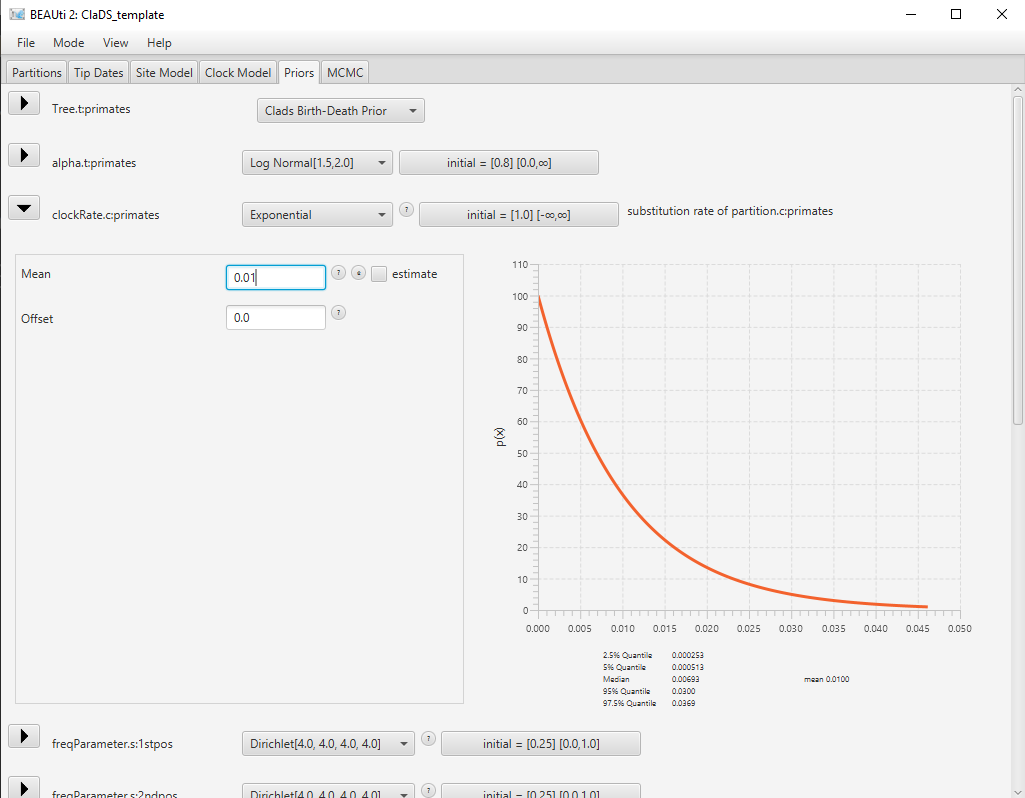
\includegraphics[width=0.800000\textwidth]{figures/clockprior.png}
    \caption{Setting the prior on the clock rate.}
    \label{clockPrior}
\end{figure}

\hypertarget{mcmc-options}{%
\subsubsection{MCMC options}\label{mcmc-options}}

The next step is to set the options for running the chain, in the
\textbf{MCMC} panel. We can see that several loggers are set by default:

\begin{itemize}

\item
  the regular trace log, which records the posterior, likelihood and
  prior, as well as parameter values for the substitution, clock and
  tree models.
\item
  the screenlog, which shows the advancement of the chain to the screen.
\item
  the tree log, which will log the trees in Nexus format, with the
  estimated clock rate on each edge as metadata.
\item
  the tree rates log, which will log the trees in Nexus format, with the
  estimated birth and death rates on each edge as metadata.
\end{itemize}

This last log is specific to ClaDS. The only thing we will change here
are the names of the log files, to ensure we can find them again.
\textgreater{} Switch to the \textbf{MCMC} panel. \textgreater{} In the
\textbf{tracelog}, change the \textbf{File Name} to
\textbf{primates.log}. \textgreater{} In the \textbf{treeRatesLog},
change the \textbf{File Name} to \textbf{primates.rates.trees}.
\textgreater{}

For this tutorial, we will also adjust the chain length and sampling
frequency, in order for the inference to complete rapidly.

\begin{framed}
In the \textbf{MCMC} panel, change the \textbf{Chain Length} to
\textbf{100000}. In the \textbf{tracelog}, \textbf{treelog} and
\textbf{treeRatesLog}, change the \textbf{Log Every} to \textbf{1000}.
\end{framed}

Once all the options have been set, the final step is to save the XML.

\begin{framed}
Save the XML file as \passthrough{\lstinline!primates_clads.xml!} by
navigating to \textbf{File \textgreater{} Save}.
\end{framed}

\hypertarget{running-the-analysis-in-beast2}{%
\subsection{Running the analysis in
BEAST2}\label{running-the-analysis-in-beast2}}

\begin{framed}
Start \textbf{BEAST2} and choose the file
\passthrough{\lstinline!primates_clads.xml!}. Hit \textbf{Run} to start
the analysis.
\end{framed}

We can already see that running the ClaDS model is quite slow. In
general, ClaDS is an expensive model to run due to its complexity, as it
requires the birth rate and/or the death rate to be resampled for each
edge of the phylogeny. Note also that having a low sampling probability
increases the computational cost of accounting for all possible
histories in the unsampled parts of the tree, and so will result in
slower inferences. In a real analysis, we could use for instance a
starting tree to make sure that the inference starts in a good place,
which should help the chain to converge faster.

\hypertarget{analyzing-the-output}{%
\subsection{Analyzing the output}\label{analyzing-the-output}}

\hypertarget{output-files}{%
\subsubsection{Output files}\label{output-files}}

Our run has generated 3 different files:

\begin{itemize}

\item
  \passthrough{\lstinline!primates.log!} which is the general trace log.
\item
  \passthrough{\lstinline!primates.trees!} and
  \passthrough{\lstinline!primates.rates.trees!} which recorded the
  sampled trees in Nexus format.
\end{itemize}

Note that our shortened analysis has not converged (as can easily be
seen when importing the log file into Tracer). If you prefer you can
analyze the pre-made log and tree files provided in this tutorial, which
have been run for longer.

\hypertarget{analyzing-the-log-files}{%
\subsubsection{Analyzing the log files}\label{analyzing-the-log-files}}

We will use the software Tracer to analyze the log file. We can see in
particular the posterior distribution of the different parameters of the
ClaDS model: the birth rate at the root
\passthrough{\lstinline!lambda_0!}, the trend
\passthrough{\lstinline!alpha!} and variance
\passthrough{\lstinline!sigma!} of the lognormal distribution used to
sample the birth rate and the \passthrough{\lstinline!turnover!} which
gives the ratio of death rates to birth rates.

One metric of interest reported by ClaDS is the mean deviation between
the rate of an edge and the rate of its parent age, which is given by
\passthrough{$ m = \alpha \times exp(\sigma ^2 /2) $}.
If the mean deviation is above 1, then the general trend is for rates to
increase from the root towards the tips of the phylogeny, whereas if the
mean deviation is below 1, the general trend is a decrease in rates from
the root to the tips. This measure is stored by ClaDS in the log file as
\passthrough{\lstinline!augTree.mB!} for the birth rates, and
\passthrough{\lstinline!augTree.mD!} for the death rates. Here we have
parametrized the death rates using a fixed turnover, so only the mean
deviation in birth rates appears in the log (Figure \ref{mB}).

\begin{figure}
    \centering
    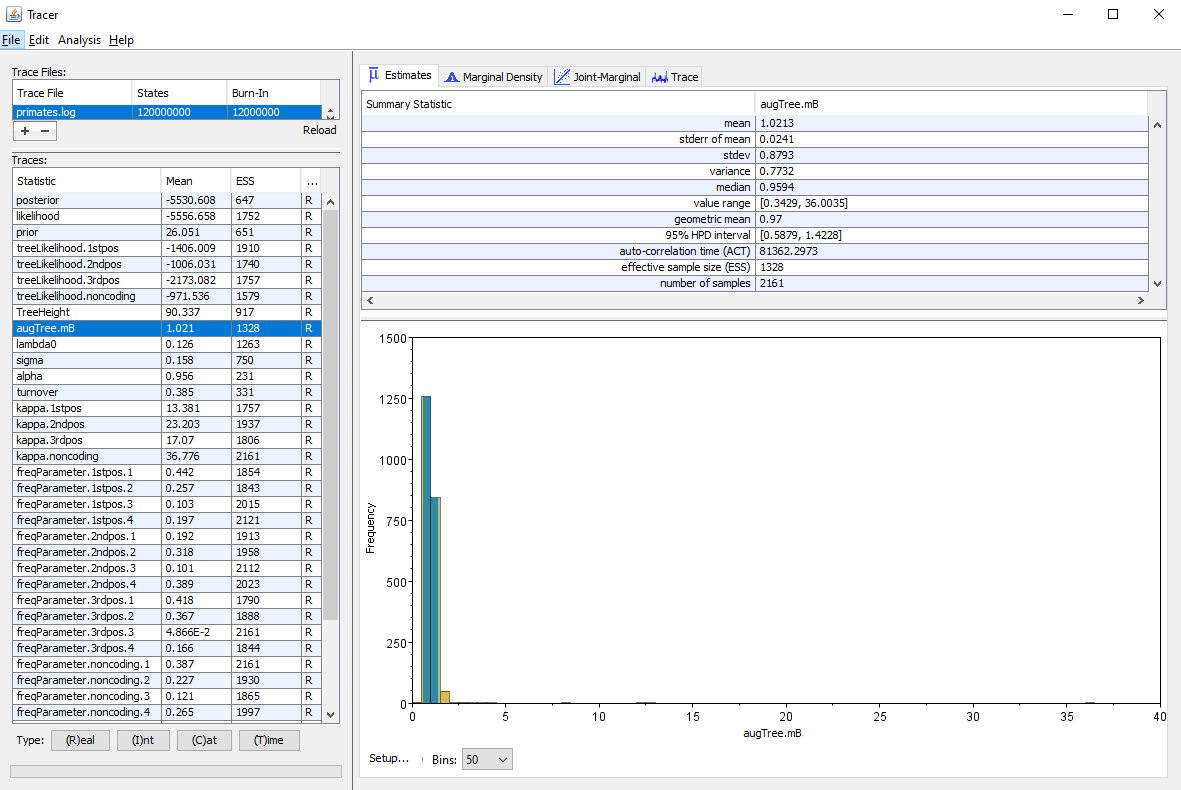
\includegraphics[max width=\textwidth, max height=0.9\textheight]{figures/tracer_mB.png}
    \caption{Estimated posterior distribution of the mean deviation in birth rates, as shown in Tracer.}
    \label{mB}
\end{figure}

\hypertarget{analyzing-the-trees}{%
\subsubsection{Analyzing the trees}\label{analyzing-the-trees}}

Another way to visualize the results is to look at the rates as plotted
on the tree. We can use TreeAnnotator to build an MCC tree from the tree
log in the file \passthrough{\lstinline!primates.rates.trees!}. Since we
also logged the birth and death rates for each edge in the tree log,
these parameters will also be summarized along with the tree.

\begin{framed}
Start \textbf{TreeAnnotator} and set the input tree to the tree file
\passthrough{\lstinline!primates.rates.trees!}. The burn-in percentage
is set to 10\% by default. Give a name to the output file, for instance
\passthrough{\lstinline!primates.MCC.tre!}.

Finally, click \textbf{Run} to start the summary.
\end{framed}

The MCC tree can be loaded into any tree visualization software, such as
FigTree or IcyTree, however these tools are designed to plot discrete
characters, and do not perform as well with a continuous character like
the birth rate. We are going to use the R script provided in this
tutorial \passthrough{\lstinline!plot_MCC.R!}. This script takes as
input the MCC tree file and an output file to store the plot, and it
will plot the MCC tree with edges coloured by the median estimates of
the birth and death rates. Run the following commands in an R console to
create the plots:

\begin{lstlisting}[language=R]
source("plot_MCC.R")
MCC_colour_plot("primates.MCC.tre", plotfile = "primates_MCC.pdf")
\end{lstlisting}

Figure \ref{mcc_birth} and Figure \ref{mcc_death} show the resulting
plots for the birth rate and the death rate, respectively.

\begin{figure}
    \centering
    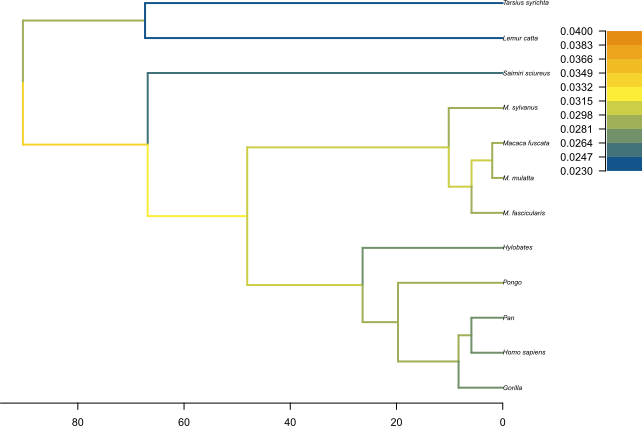
\includegraphics[max width=\textwidth, max height=0.9\textheight]{figures/mcc_birth.png}
    \caption{MCC tree with edges coloured by the median birth rate.}
    \label{mcc_birth}
\end{figure}

\begin{figure}
    \centering
    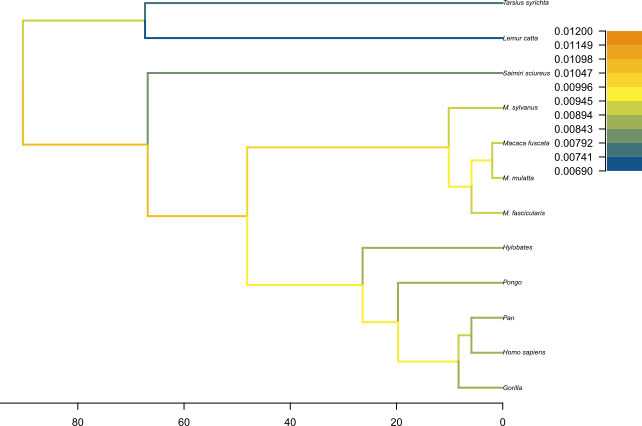
\includegraphics[max width=\textwidth, max height=0.9\textheight]{figures/mcc_death.png}
    \caption{MCC tree with edges coloured by the median death rate.}
    \label{mcc_death}
\end{figure}

We can see .

\begin{framed}
\textbf{Topic for discussion:} Do you think the pattern of birth and
death rates shown in this picture is real? Are there any other factors
in our dataset which could explain it?
\end{framed}

\hypertarget{useful-links}{%
\section{Useful Links}\label{useful-links}}

\begin{itemize}

\item
  \href{http://www.beast2.org/book.html}{Bayesian Evolutionary Analysis
  with BEAST 2} \citep{BEAST2book2014}
\item
  BEAST 2 website and documentation: \url{http://www.beast2.org/}
\item
  BEAST 1 website and documentation: \url{http://beast.bio.ed.ac.uk}
\item
  Join the BEAST user discussion:
  \url{http://groups.google.com/group/beast-users} \clearpage
\end{itemize}

\hypertarget{relevant-references}{%
}

\clearpage

%%%%%%%%%%%%%%%%%%%%%%%
% Tutorial disclaimer %
%%%%%%%%%%%%%%%%%%%%%%%
% Please do not change the license
% Add the author names and relevant links
% Add any other aknowledgments here
\href{http://creativecommons.org/licenses/by/4.0/}{
\includegraphics[scale=0.8]{figures/ccby.pdf}} This tutorial was written by Joëlle
Barido-Sottani for \href{https://taming-the-beast.github.io}{Taming the BEAST} and is licensed under a \href{http://creativecommons.org/licenses/by/4.0/}{Creative Commons Attribution 4.0 International License}. 


%%%%%%%%%%%%%%%%%%%%
% Do NOT edit this %
%%%%%%%%%%%%%%%%%%%%
Version dated: \today



\newpage

%%%%%%%%%%%%%%%%
%  REFERENCES  %
%%%%%%%%%%%%%%%%

\printbibliography[heading=relevref]


\end{document}